\chapter{Project development}
\label{chapter6}

In this chapter we will discuss and deepen in all of the tasks and subprocesses that took part in the completion of this project. We will also thoroughly detail all of the steps that were followed in order to complete these steps and materialize the mobile application.

\section{Project creation}

In order to create a Flutter project, we need to make use of the Android Studio IDE with the Flutter plugin installed (for further development, we prefer VS Code due to its simplicity). The assistant for creating a new project is shown in Figure \ref{fig:project-creation}.

\begin{figure}[h]
  \centering
  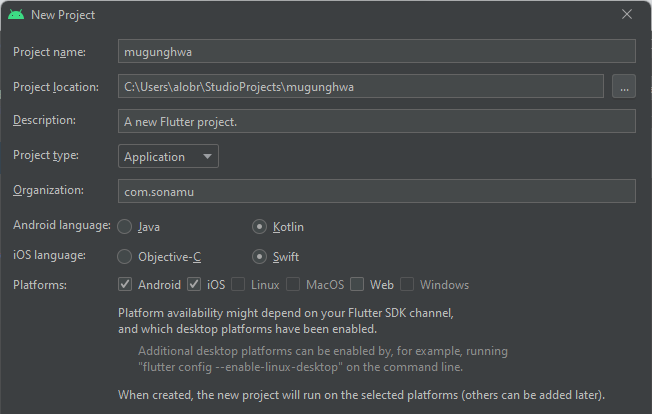
\includegraphics[width=0.75\textwidth]{Figures/project-creation.png}
  \caption{
    Creating a project in Android Studio
  }
  \label{fig:project-creation}
\end{figure}

On this screen, we need to select a project name as well as an organization. These details are relevant as they will constitute the package name. The Android and iOS languages are not important in this case, since one of the advantages of using Flutter is that only one codebase in Dart will need to be maintained for both plaforms. After clicking on "Finish", the file structure for the project will be generated.

\clearpage
\section{File structure}

Before describing the implementation of the different components of the application, we will first briefly describe the structure of all of the files in the project, excepting any automatically generated files. This structure can be seen below on Figure \ref{fig:file-structure}.

\begin{figure}[h]
  \centering
  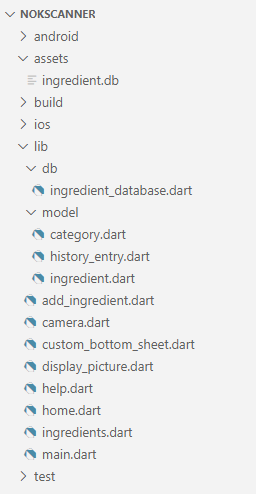
\includegraphics[width=0.5\textwidth]{Figures/file_structure.png}
  \caption{
    File structure of the Flutter project
  }
  \label{fig:file-structure}
\end{figure}

The code has been modularized mainly according to elements of the interface, dedicating a file to each of the screens or components. As well as these files on the root of \texttt{lib}, we have the folder \texttt{db} containing the files relatives to the database connection and CRUD operations. Finally, the folder \texttt{model} contains the data models for the different classes that mirror entries of the database.

\section{Camera}

One of the first things we need to figure out in order to build an app that is centered around a scanner feature is how to properly access and integrate the device camera. This is straightforward to implement if we access the default camera on the phone, but for this project we would like to implement a camera preview inside the interface of our own application.

To accomplish this, we will make use of the \texttt{camera} plugin, which offers an array of methods to access and control the device camera. There are multiple parts of the code where \texttt{camera} methods needed to be implemented, so we have selected one of them as an example for this section. In the code below (Listing \ref{lst:camera}) we can see the implementation to take a picture and forward the picture to the results screen when pressing the floating action button on the screen.

\begin{code}
\begin{minted}[
breaklines,
frame=lines,
framesep=2mm,
baselinestretch=1.2,
fontsize=\footnotesize,
linenos
]{dart}
floatingActionButton: FloatingActionButton(
  onPressed: () async {
    await _initializeControllerFuture;
    final image = await _controller.takePicture();
    _controller.setFlashMode(FlashMode.off);
    setState(() {
      flash = false;
    });

    await Navigator.of(context).push(
      MaterialPageRoute(
        builder: (context) => DisplayPictureScreen(
          imagePath: image.path,
        ),
      ),
    );
  },
)

\end{minted}
\caption{Code to take a picture and send it to the next screen}
\label{lst:camera}
\end{code}
\vskip\baselineskip

Upon pressing the button, the controller is initialized if not already present, the \texttt{takePicture()} method of the controller is called and the flash is turned off if it was previously on. Then, \texttt{DisplayPictureScreen} is pushed into the view and the image path is passed to it.

\section{Optical character recognition}

In order to implement optical character recognition in our project, we chose to integrate the ML Kit SDK into our project. ML Kit is Google's standalone library to implement machine-learning related solutions in mobile devices. Though it was previously integrated into the Firebase platform, it has since been split into the cloud-based version (Firebase ML) and the on-device and standalone version that we will use (ML Kit). One of the main reasons for choosing ML Kit over Firebase ML is its ability to function offline, which is deemed a desirable feature since travellers to a foreign country may not have access to data coverage.

ML Kit supports only native Android projects and does not offer any official integration with Flutter projects. There is, however, some Flutter implementations of the standalone ML Kit available as community packages in the Pub package repository. We will make use of the \texttt{google\_ml\_kit} package since it has been updated to also implement the Text Recognition v2 feature, which provides the OCR models to work with several non-Latin scripts including \textit{hangeul}.

To incorporate the \texttt{google\_ml\_kit} package to our project, we can simply add its name and version to the \texttt{pubspec.yaml} file which logs every dependency along with other general aspects of the app. In the Listing \ref{lst:dependencies} we can see part of the contents of this file, showing the addition of the \texttt{google\_ml\_kit} package along with every other dependency used in the project.

\begin{code}
\begin{minted}[
breaklines,
frame=lines,
framesep=2mm,
baselinestretch=1.2,
fontsize=\footnotesize,
linenos
]{yaml}
dependencies:
  flutter:
    sdk: flutter

  google_ml_kit: ^0.7.3
  camera: 0.8.1+7
  path_provider: ^2.0.7
  path: ^1.8.0
  image_picker: ^0.8.4+4
  sqflite: ^2.0.1
  http: ^0.13.4
  flutter_typeahead: ^3.2.4
\end{minted}
\caption{Dependencies of the Flutter project}
\label{lst:dependencies}
\end{code}
\vskip\baselineskip

Once we have added the required dependency, we can start working on the OCR code to recognize and extract the raw text from a given image, which is fairly straightforward. In Listing \ref{lst:ml-kit} we can see a minimal working example similar to the one coded in our application. 

\begin{code}
\begin{minted}[
breaklines,
frame=lines,
framesep=2mm,
baselinestretch=1.2,
fontsize=\footnotesize,
linenos
]{dart}
import 'package:google_ml_kit/google_ml_kit.dart';

Future<String> recognizeText(String imagePath) async {
  final inputImage = InputImage.fromFilePath(imagePath);

  final textDetector = GoogleMlKit.vision.textDetectorV2();
  final recognisedText = await textDetector.processImage(inputImage,
      script: TextRecognitionOptions.KOREAN);

  textDetector.close();

  return recognisedText.text;
}
\end{minted}
\caption{Example of OCR implementation}
\label{lst:ml-kit}
\end{code}
\vskip\baselineskip

As shown, after importing the package, we load the image from its corresponding file path. Then, we create a \texttt{TextDetectorV2} object that supports Korean language and we extract the recognised text using the asynchronous method \texttt{processImage} which takes both the input image and the desired script. Finally, we can close the text detector and return the text attribute of our \texttt{RecognisedText} object, which is a string containing all of the text identified in the image.

\section{Translation}

Although our application makes use of an ingredient database which includes the Korean-English translation for all of the terms, we still need a separate translation service for two reasons. First, there may be terms that escape the scope of our dictionary, and the user needs a backup solution for those cases. Second, we want the app to provide a translation of the scanned ingredients list to give the user some means of double-checking in case of doubt.

Initially, we intended to make use of the standalone translation service included in the already present \texttt{google\_ml\_kit} package, in order to take advantage of the offline functionality. However, since a list of ingredients may use complex or scientific terms, and the whole translation is based of a small and standalone model, the results provided were underwhelming.

Other alternatives like implementing an online translation API also have its downsides, mainly a hard limit on the amount of text to be translated daily or monthly without incurring on additional costs. Because of this, and in order to provide at least some basic functionality when the device is offline, it was decided to implement both systems into the project.

\subsection{ML Kit translation}

Since we already added the required dependency, the implementation of the translation service is reduced to making use of the available functions. Listing \ref{lst:ml-kit-translate} shows the base code for translating a string of text from English to Korean. 

\begin{code}
\begin{minted}[
breaklines,
frame=lines,
framesep=2mm,
baselinestretch=1.2,
fontsize=\footnotesize,
linenos
]{dart}
import 'package:google_ml_kit/google_ml_kit.dart';

Future<String> translateTextOffline(String text) async {
  final translateLanguageModelManager =
      GoogleMlKit.nlp.translateLanguageModelManager();

  try {
    await translateLanguageModelManager.downloadModel('en'); // English
    await translateLanguageModelManager.downloadModel('ko'); // Korean
  } catch (e) {
    print(e.toString());
  }

  final onDeviceTranslator = GoogleMlKit.nlp.onDeviceTranslator(
      sourceLanguage: TranslateLanguage.KOREAN,
      targetLanguage: TranslateLanguage.ENGLISH);

  var translatedText =
      await onDeviceTranslator.translateText(text);

  onDeviceTranslator.close();

  return translatedText;
}
\end{minted}
\caption{ML Kit's translation implementation}
\label{lst:ml-kit-translate}
\end{code}
\vskip\baselineskip

First, we create a \texttt{translateLanguageModelManager} and attempt to retrieve the models for English and Korean in case they are not already present. With the models loaded, we create an \texttt{onDeviceTranslator} with Korean as a source language and English as a target language. We can then run the translation function with our input text, close the translator, and return the translated text.

\subsection{Papago API translation}

The Papago API is a third-party solution that represents an alternative to the above mentioned ML Kit standalone service. This  API is offered by one of the most widely used translation tools in South Korea, and its free to use up to 10000 characters per day.

In order to integrate this API into our mobile application, the first step is signing up on the Naver developers platform\footnote{Available at: \url{https://developers.naver.com/}}. Upon registering as a developer, we are able to access a dashboard panel, which can be seen in Figure \ref{fig:papago-dashboard}, where we can apply for access to any of our applications. In order to apply, a small form and statement of purpose needs to be filled with the package name of the app, a brief statement of purpose, whether its destined for commercial or educational use, etc.

\begin{figure}[h]
  \centering
  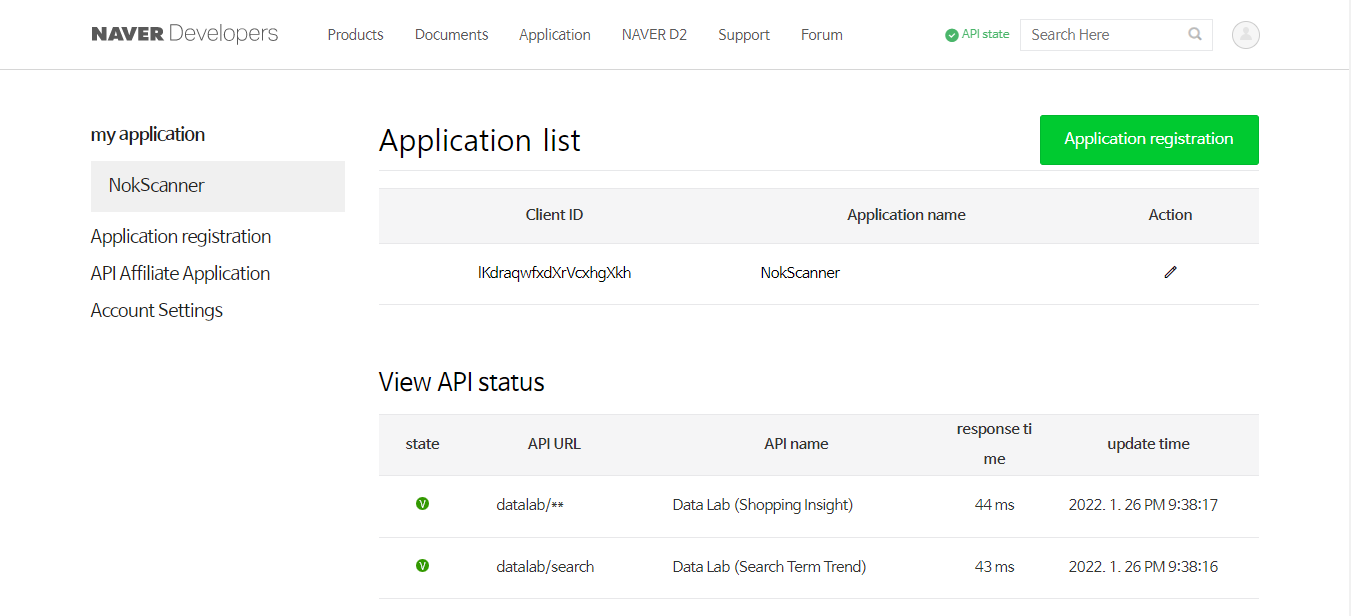
\includegraphics[width=\textwidth]{Figures/papago-dashboard.png}
  \caption{
    Naver Developer's platform (translated)
  }
  \label{fig:papago-dashboard}
\end{figure}

After getting approval for API usage in or application, we are provided with a client ID and secret that grants access to the service. At this point, we can start implementing the code in our Flutter project. To make it work, we will also need to make use of the \texttt{http} package in order to send and process HTTP requests. A code sample for translating text using this API is shown in Listing \ref{lst:papago-translate}.

\begin{code}
\begin{minted}[
breaklines,
frame=lines,
framesep=2mm,
baselinestretch=1.2,
fontsize=\footnotesize,
linenos
]{dart}
import 'package:http/http.dart' as http;

Future<String?> translateTextPapago(String text) async {
  String clientId = "lKdraqwfxdXrVcxhgXkh";
  String clientSecret = "**********";
  String contentType = "application/x-www-form-urlencoded; charset=UTF-8";
  String _url = "https://openapi.naver.com/v1/papago/n2mt";

  http.Response trans = await http.post(
    Uri.parse(_url),
    headers: {
      'Content-Type': contentType,
      'X-Naver-Client-Id': clientId,
      'X-Naver-Client-Secret': clientSecret
    },
    body: {
      'source': "ko",
      'target': "en",
      'text': text,
    },
  );

  if (trans.statusCode == 200) {
    var dataJson = jsonDecode(trans.body);
    var resultPapago = dataJson['message']['result']['translatedText'];
    return resultPapago;
  }
}
\end{minted}
\caption{Papago API's translation implementation}
\label{lst:papago-translate}
\end{code}
\vskip\baselineskip

As shown in the code, the first step is to define variables for our API keys (the secret has been hidden for this example), as well as the content type and the URL of the API. Then, using the HTTP package, we can construct and post our request as shown, including the source and target language as well as the input text. If the response status code is 200, we can assume that it was accepted and proceed to decode and extract the translated text from the JSON answer received. Otherwise, as this function returns a nullable type, no value is returned and the outcome will be null.

\subsection{Translation merging}

Once both services are implemented, we can freely join and make use of both systems on a general function that translates a text using any of the systems depending on its availability, as shown in Listing \ref{lst:translate-join}.

\begin{code}
\begin{minted}[
breaklines,
frame=lines,
framesep=2mm,
baselinestretch=1.2,
fontsize=\footnotesize,
linenos
]{dart}
Future<String> translateText(String text) async {
  var translatedText = await translateTextPapago(recognisedText.text);
  translatedText ??=
      await translateTextOffline.translateText(recognisedText.text);

  return translatedText;
}
\end{minted}
\caption{Merging translation services}
\label{lst:translate-join}
\end{code}
\vskip\baselineskip

As seen in the code, our application will always attempt to use the online translation service first. If the status code of the response is different from 200, or if the request failed because of any other reason, the function will return a null value. The null-coalescing assignment operator \texttt{??=}, also present in other similar languages such as C\#, is an assignation that will proceed only if the left-hand operand is null. Therefore, if the online translation fails, execution will continue running the on-device translation service. In any case, only one of the functions will be run and its output string will be returned.

\section{Database}

In order to build an efficient application that can accurately identify any possible allergens, relying on translation services is not a solid choice. These services cannot identify what is a food ingredient and what is not, and may produce wildly different results depending on the surrounding text. Therefore, we need a robust data source at the core of the backend that can tell our application which Korean words are ingredients, as well as determining a single fixed English translation for all of them.

In this section we will delve into the process of finding and cleaning our dataset, constructing the data models, and implementing and connecting the system into our Flutter project.

\subsection{Obtaining the data}

For this project, we needed to find a data set that was constituted of a list of ingredients used in the manufacturing of Korean food products and that ideally also included an attribute for their English translations. After a thorough browsing of many of the Korean government sources, we found one data set that satisfied all of this criteria.

The Food Composition Database, provided by the Ministry of Food and Drug safety of South Korea, offers a comprehensible list of up to 3000 different ingredients and derived products along with their English name, category and nutritional value per 100g. This data is made available after filling a small questionnaire, as detailed in Chapter \ref{chapter5}, and is provided as an Excel file with .xls format.

The first step was manually cleaning the database out of any redundant entries. Some of the elaborated ingredients included had several entries depending on how they were manufactured or processed, for example, which may affect their nutritional value but usually has no effect on allergies or food intolerances. Therefore, these entries were merged and several accepted Korean names were provided when needed. Also, every unneeded column was removed from the spreadsheet. After this process, the number of total entries was reduced from 3113 to 1242. A sample of the data set after the cleaning process is shown in Figure \ref{fig:data-dblike}.

\begin{figure}[h]
  \centering
  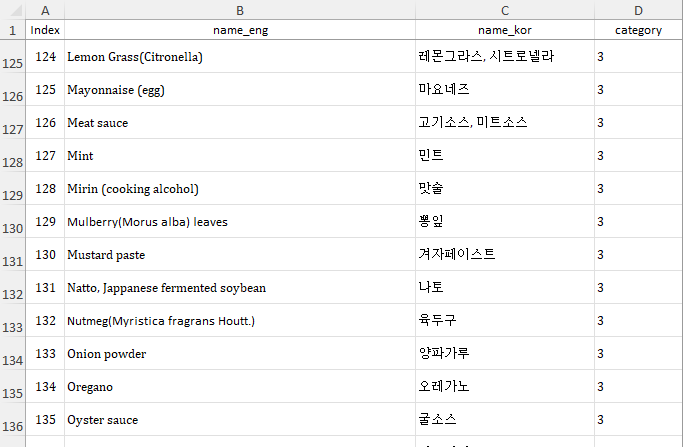
\includegraphics[width=0.65\textwidth]{Figures/data-dblike.png}
  \caption{
    Sample data after cleaning
  }
  \label{fig:data-dblike}
\end{figure}

\subsection{Building the database}

Once we have arranged the data that will be utilized in the backend of our application, the next step is transporting it from the Excel file to a data structure comprehensible by any of the database engines available. For this project we will make use of SQLite along with the SQFLite Flutter plugin, since it offers a lightweight and server-less solution for storing data that fits our needs for the scale of this app.

Before getting hands into building the data model, the first step is transforming our data into a CSV (comma-separated value) file that we can easily feed into any database. This can be easily done through Excel itself, by selecting the option Save as > CSV (comma-delimited).

Once we have our CSV file ready, the next step will be creating our database SQlite database file. Although this can be entirely done using SQL syntax, we will make use of a GUI tool that will simplify many of the processes, particularly importing the data from our CVS file. This tool is DB Browser for SQLite (DB4S).

After opening DB4S and creating a new database file, the next thing we will need is creating an ingredients table to store our data. This can be done through the assistant tool shown in Figure \ref{fig:db4s-create}.

\begin{figure}[h]
  \centering
  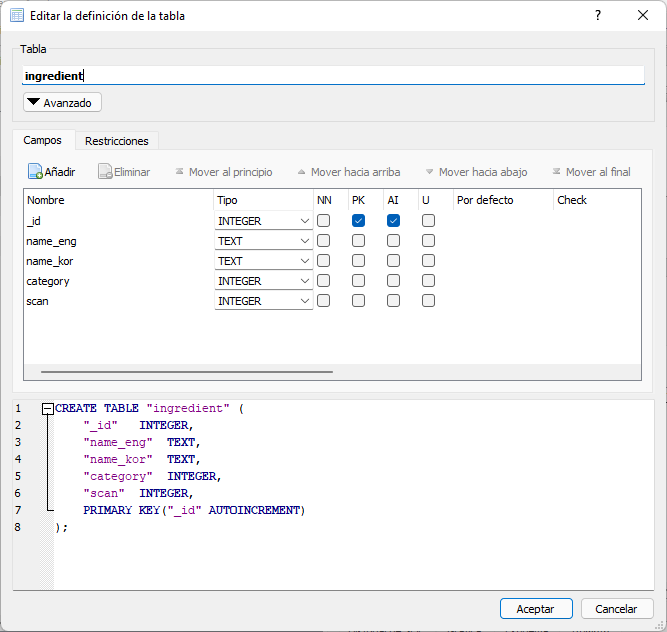
\includegraphics[width=0.65\textwidth]{Figures/db4s-create.png}
  \caption{
    Creating a new table in DB Browser for SQLite
  }
  \label{fig:db4s-create}
\end{figure}

As shown in the figure, we can add any columns we need to the table, giving them a name and a type, or setting them as primary key in the case of the ID field. The text field below shows the equivalent SQL syntax. Once we are finished creating the table, we can move our CSV data into it by importing the file. This can again be done easily using the assistant shown in Figure \ref{fig:db4s-import}

\begin{figure}[h]
  \centering
  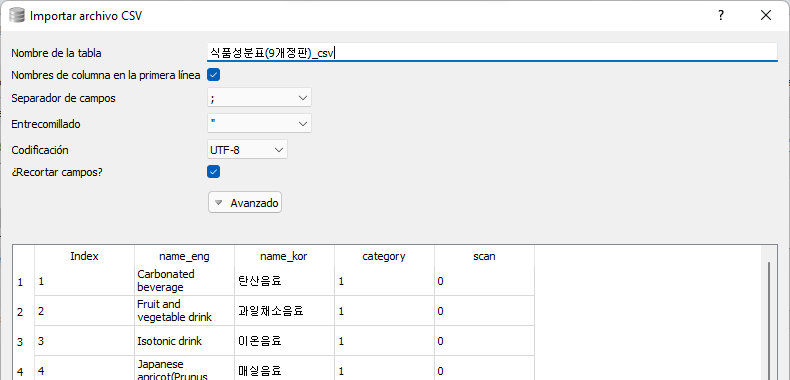
\includegraphics[width=0.50\textwidth]{Figures/db4s-import.png}
  \caption{
   Importing CVS data in DB Browser for SQLite
  }
  \label{fig:db4s-import}
\end{figure}

Now that we have a database file (.db) storing all our ingredient data and ready to use, it is time to move it to our Flutter project. As shown previously on Figure \ref{fig:file-structure}, we will store it on its own "assets" folder.

\subsection{Modelling the data}

Besides, we will need to create data models that mirror in our Flutter app the structure of the data stored in the database. In Listing \ref{lst:db-model} we can see the code for the \texttt{Ingredient} data model.

\begin{code}
\begin{minted}[
breaklines,
frame=lines,
framesep=2mm,
baselinestretch=1.2,
fontsize=\footnotesize,
linenos
]{dart}
const String tableIngredient = 'ingredient';

class IngredientFields {
  static final List<String> values = [id, nameEng, nameKor, categoryId, scan];

  static const String id = '_id';
  static const String nameEng = 'name_eng';
  static const String nameKor = 'name_kor';
  static const String categoryId = 'category_id';
  static const String scan = 'scan';
}

class Ingredient {
  final int? id;
  final String nameEng;
  final String nameKor;
  final int categoryId;
  final bool scan;

  Ingredient({
    this.id,
    required this.nameEng,
    required this.nameKor,
    required this.categoryId,
    required this.scan,
  });

  static Ingredient fromJson(Map<String, Object?> json) => Ingredient(
        id: json[IngredientFields.id] as int?,
        nameEng: json[IngredientFields.nameEng] as String,
        nameKor: json[IngredientFields.nameKor] as String,
        categoryId: json[IngredientFields.categoryId] as int,
        scan: json[IngredientFields.scan] == 1,
      );

  Map<String, Object?> toJson() => {
        IngredientFields.id: id,
        IngredientFields.nameEng: nameEng,
        IngredientFields.nameKor: nameKor,
        IngredientFields.categoryId: categoryId,
        IngredientFields.scan: scan ? 1 : 0,
      };

  Ingredient copy({
    int? id,
    String? nameEng,
    String? nameKor,
    int? categoryId,
    bool? scan,
  }) =>
      Ingredient(
        id: id ?? this.id,
        nameEng: nameEng ?? this.nameEng,
        nameKor: nameKor ?? this.nameKor,
        categoryId: categoryId ?? this.categoryId,
        scan: scan ?? this.scan,
      );
}
\end{minted}
\caption{Data model for Ingredient}
\label{lst:db-model}
\end{code}
\vskip\baselineskip

The code above defines the attributes that the \texttt{Ingredient} object will have in our Flutter project, and matches each of these attributes with a column of the \texttt{Ingredient} table in our database. It also defines additional methods to convert to JSON, retrieve from JSON, and copy the object. We will make use of these methods and pairings between class attributes and column names at the next step, connecting the database to our project.

\subsection{Connecting the database}

In order to connect the database and implement any CRUD operation needed, we will create a new separate class dedicated to all the database-related implementation. The first method we will need is one that will access the app database, or retrieve the data from the .db file if it is the first time running the app. The code for this method is listed on Listing \ref{lst:db-init}.

\begin{code}
\begin{minted}[
breaklines,
frame=lines,
framesep=2mm,
baselinestretch=1.2,
fontsize=\footnotesize,
linenos
]{dart}
Future<Database> _initDB(String filePath) async {
  final dbPath = await getDatabasesPath();
  final path = join(dbPath, filePath);

  var exists = await databaseExists(path);
  if (!exists) {
    try {
      await Directory(dirname(path)).create(recursive: true);
    } catch (_) {}

    ByteData data = await rootBundle.load(join("assets", "ingredient.db"));
    List<int> bytes =
        data.buffer.asUint8List(data.offsetInBytes, data.lengthInBytes);

    await File(path).writeAsBytes(bytes, flush: true);
  }

  return await openDatabase(path);
}

\end{minted}
\caption{Initializing the database}
\label{lst:db-init}
\end{code}
\vskip\baselineskip

The implementation of this method is quite self-explanatory. It will check if a database already exists at the defined path, and if it does not it will create a new one by copying the file in \texttt{assets/ingredients.db} to the databases path. Then, it will open the database and return the execution.

Finally, the only thing left to do is defining as much CRUD operations as we will need for the implementation of the logic of our application. Several tables, models and CRUD operations were implemented through the development of the project. As an example, the operation to retrieve all ingredients that are currently being scanned (scan = 1) is shown in Listing \ref{lst:crud}.

\begin{code}
\begin{minted}[
breaklines,
frame=lines,
framesep=2mm,
baselinestretch=1.2,
fontsize=\footnotesize,
linenos
]{dart}
Future<List<Ingredient>> readAllScanIngredient() async {
  final db = await instance.database;
  final result = await db.query(tableIngredient,
      where: '${IngredientFields.scan} = 1');
  return result.map((json) => Ingredient.fromJson(json)).toList();
}
\end{minted}
\caption{Example of CRUD method}
\label{lst:crud}
\end{code}
\vskip\baselineskip

As seen on the code, in any of the CRUD operations the database is accessed using \texttt{instance.database}. Then, it can be queried using standard SQL syntax or passing all the necessary information (table, where clause, order...) as parameters to the \texttt{db.query} function. Finally the results retrieved as a JSON are converted to \texttt{Ingredient} objects using the \texttt{fromJson} method and the list of ingredients that matches the query is returned.

After adding all the needed models, connections and CRUD methods to our Flutter project, we are finished implementing the data structure that supports the backend of the app. The proposed database architecture employed for the mobile application can be seen on Figure \ref{fig:db-diagram}.

\begin{figure}[h]
  \centering
  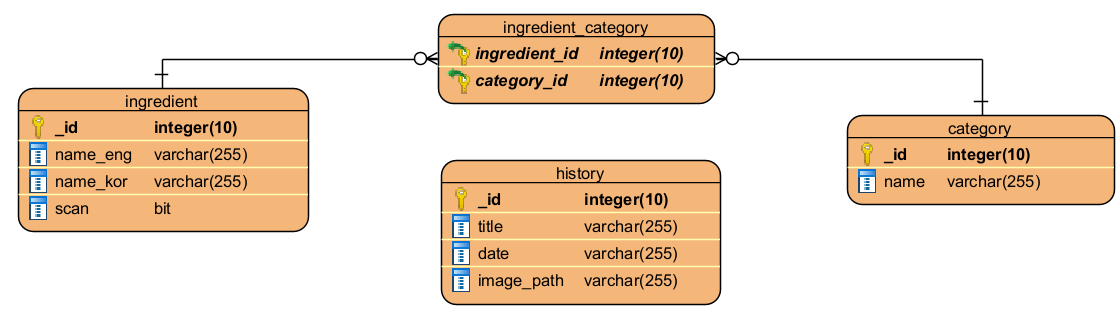
\includegraphics[width=\textwidth]{Figures/db_diagram.png}
  \caption{%
    Entity-relationship diagram for the app database
  }
  \label{fig:db-diagram}
\end{figure}

\section{Detecting ingredients}

Now that we can access our database of ingredients from any class of our Flutter project, we can start implementing the function dedicated to detect matches between the text recognized by the OCR system and the ingredients specified by the user to be flagged.

Because false positives are greatly preferable over false negatives, the algorithm will be coded in the most lax way possible so as to detect any combination of characters that match any of the Korean names of any unwanted ingredient. This way, even if the name of any unwanted ingredient appears inside of a larger word, it will still be flagged. This behaviour is by design since Korean language, much like Turkish or Japanese, is agglutinative, and therefore a large combination of compound words can be constructed by adding prefixes and suffixes to a smaller stem. The function dedicated to finding any matches across the text and the ingredient blacklist is shown in Listing \ref{lst:matcher}.

\begin{code}
\begin{minted}[
breaklines,
frame=lines,
framesep=2mm,
baselinestretch=1.2,
fontsize=\footnotesize,
linenos
]{dart}
Future<List<Ingredient>> matcher(String text) async {
  List<Ingredient> ingredients =
      await IngredientDatabase.instance.readAllScanIngredient();
  List<Ingredient> matches = <Ingredient>[];

  for (final ing in ings) {
    List<String> flags = ing.nameKor.split(', ');
    for (final flag in flags) {
      if (text.contains(flag) && !matches.contains(ing)) {
        matches.add(ing);
      }
    }
  }

  return matches;
}
\end{minted}
\caption{Matching algorithm}
\label{lst:matcher}
\end{code}
\vskip\baselineskip

The algorithm shown in the code snippet will first load the list of ingredients making use of the read operation that was shown in the previous section (Listing \ref{lst:crud}). Another list of ingredients is defined to store all of the unwanted ingredients that are recognized within the text. Then, the function will simply iterate through each an every unwanted ingredient, retrieve all of its possible Korean names (flags) by splitting them from a comma-separated list, and check if any of these flags is contained in the text. If the flag is found, the ingredient is added to the matches list. After finishing iterating, the matches list is returned.

\section{User interface}

Designing and implementing the different screens and navigation routes between them was one of the largest tasks from the development phase, with most lines of code being dedicated to organize the different elements of the interface. Since Flutter lacks a visual editor or storyboard unlike other frameworks like Swift or Android native, all of the components have to be implemented programatically.

In this section, we will have a brief overview of how this is done in Flutter, as well as providing some code examples that introduce the syntax of Flutter's widget architecture.

\subsection{Navigation}

Navigation in Flutter is handled using a stack architecture. When a new view is accessed from a previous one, it is pushed on top of the navigation stack. If we want to go back to the previous view, we can simply pop the current top of the navigation stack and we will go back at the parent view. An example of the code to perform these operations can be found in Listing \ref{lst:nav-stack}.

\begin{code}
\begin{minted}[
breaklines,
frame=lines,
framesep=2mm,
baselinestretch=1.2,
fontsize=\footnotesize,
linenos
]{dart}
// Push DisplayPictureScreen view into the navigator stack
Navigator.of(context).push(
  MaterialPageRoute(
    builder: (context) => DisplayPictureScreen(
      // Pass image.path to DisplayPictureScreen view
      imagePath: image.path,
    ),
  ),
);

// Pop to parent view
Navigator.pop(context);
\end{minted}
\caption{Code for pushing and popping views in the stack}
\label{lst:nav-stack}
\end{code}
\vskip\baselineskip

\subsection{Widgets}

Interfaces in Flutter are structured in a hierarchy of components called widgets. That way we can build custom elements for the views in our app by composing several base widgets together until achieving the desired look and behaviour. In the following example from the app (Listing \ref{lst:widget}), we can see a parent widget composed of up to 3 layers of other widgets.

\begin{code}
\begin{minted}[
breaklines,
frame=lines,
framesep=2mm,
baselinestretch=1.2,
fontsize=\footnotesize,
linenos
]{dart}
Expanded( // Expanded widget - L0
  flex: 16,
  child: Column( // Column widget - L1
    children: [
      TextField( // TextField widget - L2
        controller: textController,
        style: Theme.of(context).textTheme.headline5),
      Text(date, style: Theme.of(context).textTheme.subtitle1), // Text widget - L2
      const SizedBox(height: 16), // SizedBox widget - L2
      Card( // Card widget - L2
        color: found.isEmpty ? Colors.lightGreen : Colors.red,
        child: Text( // Text widget - L3
          found.isEmpty
              ? "\n✅ 0 unwanted ingredients found\n"
              : "\n❎ ${found.length} unwanted ingredients found\n",
          style: Theme.of(context).textTheme.headline6,
          textAlign: TextAlign.center))])),
\end{minted}
\caption{Code for composed widget}
\label{lst:widget}
\end{code}
\vskip\baselineskip

The resulting widget can be seen in Figure \ref{fig:widget}.

\begin{figure}[h]
  \centering
  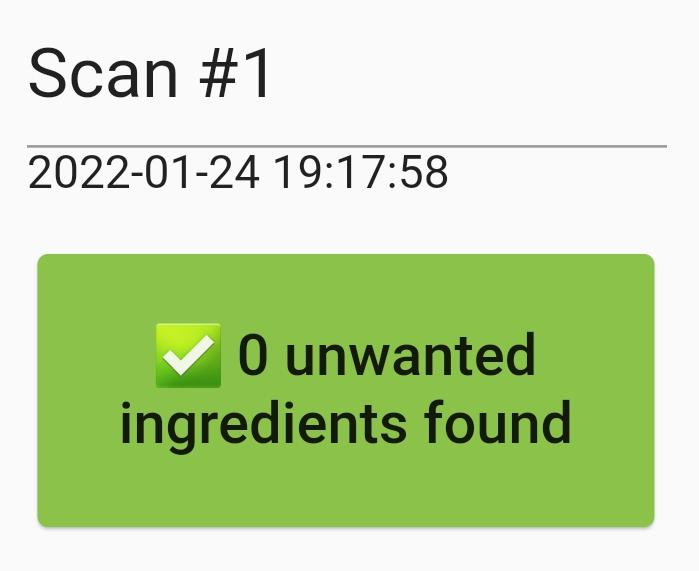
\includegraphics[width=0.4\textwidth]{Figures/widget.png}
  \caption{%
    Widget example
  }
  \label{fig:widget}
\end{figure}

\subsection{Use case diagram}

In order to better visualize the structure navigation routes across the different screens of the finished application's user interface, a use case diagram is provided in Figure \ref{fig:use-case-diagram}.

\begin{figure}[h]
  \centering
  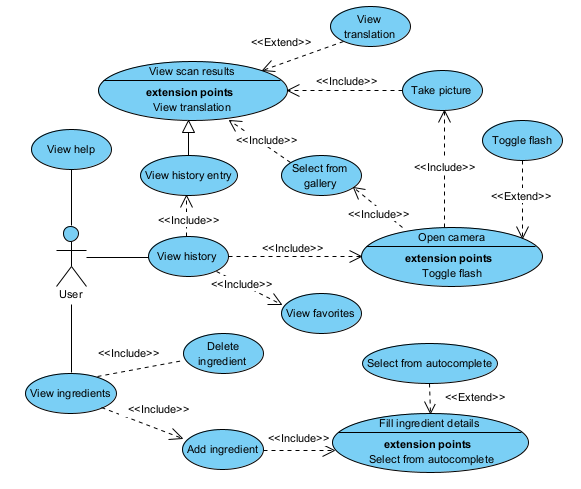
\includegraphics[width=\textwidth]{Figures/use_case_diagram.png}
  \caption{%
    Use case diagram
  }
  \label{fig:use-case-diagram}
\end{figure}

